\documentclass{sigkddExp}

\begin{document}
%
% --- Author Metadata here --- -- Can be completely blank or contain 'commented'
% information like this... \conferenceinfo{WOODSTOCK}{'97 El Paso, Texas USA} %
% If you happen to know the conference location etc. \CopyrightYear{2001} %
% Allows a non-default  copyright year  to be 'entered' - IF NEED BE.
% \crdata{0-12345-67-8/90/01}  % Allows non-default copyright data to be
% 'entered' - IF NEED BE. --- End of author Metadata ---

\title{Covid-19 X-ray Image Classification}
%\subtitle{[Extended Abstract]

\numberofauthors{4}

\author{\alignauthor Maneesh Kumar Singh\\
    \affaddr{University of Illinois at Urbana-Champaign}\\
    \email{mksingh4@illinois.edu}
    \alignauthor Raman Walwyn-Venugopal\\
    \affaddr{University of Illinois at Urbana-Champaign}\\
    \email{rsw2@illinois.edu}
    \alignauthor Satish Reddy Asi\\
    \affaddr{University of Illinois at Urbana-Champaign}\\
    \email{sasi2@illinois.edu}
    \alignauthor Srikanth Bharadwaz Samudrala\\
    \affaddr{University of Illinois at Urbana-Champaign}\\
    \email{sbs7@illinois.edu}
}

\date{28 March 2021}
\maketitle
\begin{abstract}
    Detecting COVID-19 using Chest X-Ray (CXR) images is becoming increasingly
    popular in deep learning research. When training deep neural networks, large
    and balanced datasets are preferred. However, since COVID-19 is new, there
    are a limited number of CXR images available which results in a challenge
    for training deep neural networks. Existing research has shown different
    approaches to address this imbalanced data issue. Two notable studies are
    FLANNEL[5]  an ensemble based network with focal loss and a patch-based
    classifier[6]  that works on segmented versions of the lung contours. We
    propose merging these two concepts together to improve performance of
    detecting COVID-19 in CXR images.

    Use segmentation networks to create masks for the lungs as a pre-processing
    step. Replace base models in FLANNEL with patch-based classifiers that take
    the image and respective mask as their input. The patch-based classifiers
    will be used as the ensemble.

    We are able to reproduce FLANNEL and base models results using the updated
    datasets. We were also able to reproduce patch-based classification using
    X-ray images. We also created a segmentation network that can produce masks
    of the lung contours for CXR images. We successfully used this segmentation
    network to produce masks of the CXR images in the updated FLANNEL datasets.

    We saw improvement in metrics when training the base models and FLANNEL
    ensemble in detecting COVID-19 images. Since no parameters were changed, we
    suspect that this is due to the increase of COVID-19 images for the dataset
    in comparison to when the FLANNEL paper was written. We are in the process
    of training the patch-based classifiers to use as the base models for the
    ensemble.

    With the success of performing segmentation on the dataset and the increased
    performance of the original base models due to the increased dataset size,
    we are hoping that this will lead to a further improvement once we finalize
    the patch-based classifiers. Our optimism is due to the patch-based
    classifiers outperforming their “global” counterparts that processed the
    whole non-segmented image as discussed by Park et. al [6].

\end{abstract}

\section{Introduction}
The sudden outbreak of an unexplained pneumonia found in Wuhan, China [1] was
caused by a new coronavirus infection named nCOVID-19 (Novel CoronaVirus Disease
2019). This pandemic has ravaged the world on an unprecedented scale. By April
2021, 141 million people have been infected and there have been 3.01 million
deaths. The related studies reveal that infected patients exhibit distinct
radiographic visual characteristics along with fever, dry cough, fatigue,
dyspnea, etc. Chest X-Ray (CXR) is one of the important, non-invasive [2]
clinical diagnosis tools that helps to detect COVID-19 and other pneumonia for
affected patients.

Using deep learning for X-ray classification is an ongoing research area and
recently there have been promising models proposed for COVID-19 classification.
The problem that all of these models face is an imbalance dataset due to the
limited number of COVID CXR images available.

FLANNEL is a COVID-19 CXR classification model proposed by Zhi Qiao et al.
\cite{10.1093/jamia/ocaa280} that has been shown to accurately detect COVID-19
even when trained with only 100 available COVID-19 x-ray images. There are two
core components for the FLANNEL architecture, the first is that it uses an
ensemble \cite{58871} of five independent base learners that predict the
classification of the CXR. Each of the predictions are then passed through
another ensemble network to determine the final prediction classification. The
goal of the ensemble is to increase the robustness and accuracy of the network
since each base learner should capture patterns in the images independently
\cite{combine}. The second core component for the FLANNEL is its use of the
special Focal Loss \cite{lin2018focal} function, a modification of the standard
cross-entropy loss that places a focus on the imbalance negatives by applying
down-weights to well-classified examples. Focal Loss has been known to improve
performance for imbalanced datasets.

Park et. al \cite{pmid32396075} has also created a deep learning model that has
been proven to be effective on detecting COVID-19 when trained with limited
datasets. The approach taken was to first detect lung contours of the CXR and
perform segmentation. The motivation for performing segmentation first is that
the patch based model focuses on the lung area since it’s the primary region of
interest used to perform analysis.  In general, standard biomarkers
\cite{pmid32396075} from CXR images analyzed are the following
\begin{enumerate}
    \item Lung Morphology Mean Lung Intensity
    \item Standard Deviation of Lung Intensity
    \item Cardiothoracic Ratio (CTR)
\end{enumerate}

Thus it could be observed that most of the initial diagnosis is carried out from
CXR images by concentrating the lung area, that is our motivation to adopt this
thought to have the patched method integrate with Flannel approach. We also find
by doing this it makes the model less susceptible to noise happening outside the
lung region. After the lungs have been segmented, patch-based classification is
performed. Patch-based classification involves selecting random crops or patches
across the image for a set number of times and then performing classification on
each patch. Afterwards, the final prediction of the image is made by majority
voting based on the prediction of each patch. From the graphs provided in the
paper \cite{pmid32396075} by Park and Ye, it is clear that the patch-based
classification outperformed the models that used the whole image for a limited
train set data. As we have an imbalanced dataset with limited COVID 19 CXR
images, we are optimistic that utilizing patch-based classification models for
the FLANNEL ensemble with the combination of focal loss optimization would
result in a performance improvement.

Our goal is to take the novel ideas of each approach listed above with the goal
of improving performance. To accomplish this we will make modifications to the
existing FLANNEL architecture by first pre-processing the CXR images by
performing segmentation of the lung contours. Afterwards, we will then update
the independent base learners in the ensemble to be patch-based classifiers. We
call this new architecture “Patched FLANNEL”



\section{Method}

The primary objective was to improve the detection of COVID-19 in CXR images
with a multi-classifier model that can detect Normal, Pneumonia Viral, Pneumonia
Bacteria and COVID-19. The baseline we will be comparing against is the original
FLANNEL architecture. We used the same datasets that were used in the FLANNEL
paper, the COVID Chest X-ray Dataset from
\href{https://github.com/ieee8023/covid-chestxray-dataset}{GitHub} and the
\href{https://www.kaggle.com/paultimothymooney/chest-xray-pneumonia}{Kaggle
Chest X-ray} images dataset. Similar to the FLANNEL paper, we also restricted
the types of images used to anteroposterior (AP) or posteroanterior (PA). The
restricted images were then labelled into one of four categories; COVID-19,
Viral Pneumonia, Bacterial Pneumonia and Normal.

The first major data pre-processing step that we performed on our dataset was
segmentation. In order to accomplish this, we recreated the same segmentation
network that Park et al. used for their patch-based classification;
FC-DenseNet103 \cite{DBLP:journals/corr/JegouDVRB16}. We trained the
FC-DenseNet103 model using PyTroch to produce a mask of the lung contours of a
CXR image. The datasets that were used to train the segmentation network were
the Japanese Society of Radiological Technology (JSRT)
\href{http://db.jsrt.or.jp/eng.php}{dataset} which contained 247 PA CXR images
and the Segmentation in Chest Radiographs (SCR)
\href{https://www.isi.uu.nl/Research/Databases/SCR/}{database} which contains
segmentation masks for the CXR images from the JSRT dataset. The JSRT/SCR
dataset were randomly split where 80\% of images were used for training and 20\%
were used for validation; this resulted in 197 images being used for training
and 50 images being used for validation for the JSRT dataset as shown in Table
2. Since CXR images from different data sources will come in a wide variety of
formats, the JSRT dataset was pre-processed by performing data type casting to
float32, histogram equalization to adjust the contrast, gamma correction to
adjust brightness and standardizing the image size by resizing it to 256x256.
During training, the network parameters were initialized with a random
distribution and the Adam optimizer was used with an initial learning rate of
0.0001. The learning rate was decreased by a factor of 10 when there was no
improvement in the loss. The Jaccard Index (JI) was used to evaluate the model
during training since we were comparing the similarity of the mask produced by
the network to the mask provided in the SCR dataset. An early stopping strategy
was used based on the validation performance to prevent the model from
overfitting.

We then applied the trained FC-DenseNet103 segmentation model on the AP and PA
CXR images from the Covid Chest X-ray and Kaggle X-ray datasets, this resulted
in producing a mask for the lung contours for each of the images. We then split
the segmented dataset using a train-test ratio of 4:1 to randomly generate train
test splits. To ensure reporting accurate performance on the base models, we
used five fold cross validation while training.

The next improvement that we produced was creating patch-based classifiers.
Similar to the original global base models in FLANNEL, the patch base models
used were pre-trained from ImageNet to account for the small size of the
dataset. The pre-processed images were first resized to 1024x1024 to be as close
to the original pixel distribution. The masks generated from the FC-DenseNet103
segmentation model were also upsampled to 1024x1024 to match the new CXR image
size.The resized images were then masked with the lung-contours and passed as
input to the patch-based classifier. The patch-based classifier then produced k
number crops/patches of size 224x224 from the CXR. To limit patches outside the
lung area, the random points were forced to be within the lungs and the random
point was used as the center of the patch. During inference, the k should be
large enough to ensure that the lung pixels are covered multiple times. Each
patch is then fed into a network to produce a prediction. The confidence score
was calculated for each category by calculating the percentage of predictions
for each class based on the k patches. The optimization algorithm used during
training was the Adam optimizer with a learning rate of 0.00001. An early
stopping strategy based on validation performance was applied and a weight decay
and L1 regularization were used to prevent overfitting. The best model is
selected among 200 epochs training. Considerations Here are our considerations
discussed below -
\begin{itemize}
    \item The pretrained model for segmentation (FC-Densenet103) will perform
    well on the datasets used in FLANNEL[7] paper.
    \item The number of patches(K) to be 100 to start with, will be fine tuned
    after evaluating the results.
    \item The patch image size will be chosen as 224X224 initially and will be
    fine tuned after evaluating the results.
\end{itemize}
  




\begin{table}
    \caption{FC\-DenseNet103 Segmentation Training \& Validation Dataset}
    \label{table:segdata}
    \begin{tabular}{ll} \hline
        Dataset & Number of images \\ \hline
        Training & 197 \\
        Validation & 50 \\
        \hline
    \end{tabular}

\end{table}

\begin{table*}
    \centering
    \caption{Experimental data description}
    \label{table:datastats}
    \begin{tabular}{llrrrrr} \hline
        Source                                 &           & Total  & COVID-19 &
        Viral                                  & Bacterial & Normal \\ \hline
        \multirow{2}{*}{} Original data        & CCX data  & 554    & 478      &
        16                                     & 42        & 18 \\
                                               & KCX data  & 5856   & 0        &
        1493                                   & 2780      & 1583 \\
        \hline
        \multirow{2}{*}{} View Distribution    & AP view   & 6163   & 282      &
        1501                                   & 2789      & 1591 \\
                                               & PA view   & 247    & 196      &
                                               8 & 33        & 10 \\ \hline
        \multirow{3}{*}{} Training/test splits & Training  & 5127   & 378      &
        1509                                   & 2291      & 1288 \\
                                               & Testing   & 1283   & 100      &
        339                                    & 531       & 313 \\
                                               & Total     & 6410   & 478      &
        1509                                   & 2822      & 1601 \\
        \hline
    \end{tabular}\par
    \bigskip
    AP: anteroposterior; CCX: COVID Chest X-ray; COVID-19: coronavirus disease
    2019; KCX: Kaggle Chest X-ray; PA: posteroanterior.
\end{table*}



\begin{table*}
    \centering
    \caption{Performance comparison on F1 score: Class-specific F1 score is calculated using 1 class vs the rest strategy}
    \label{table:resultstats}
    \begin{tabular}{ lccccc } \hline
                      & COVID-19      & Pneumonia virus & Pneumonia bacteria &
        Normal        & Macro-F1 \\ \hline

        Densenet161   & 0.7694 (0.03) & 0.5901 (0.05)   & 0.8030 (0.01)      &
        0.8875 (0.02) & 0.7625 (0.02) \\
        InceptionV3   & 0.8938 (0.01) & 0.6413 (0.03)   & 0.8112 (0.02)      &
        0.9015 (0.03) & 0.8120 (0.02) \\
        Resnet152     & 0.8302 (0.02) & 0.6218 (0.02)   & 0.8046 (0.01)      &
        0.9080 (0.00) & 0.7911 (0.01) \\
        ResNeXt101    & 0.8197 (0.03) & 0.6151 (0.04)   & 0.8016 (0.01)      &
        0.9046 (0.01) & 0.7852 (0.02) \\
        Vgg19\_bn     & 0.8753 (0.02) & 0.6023 (0.01)   & 0.8016 (0.01)      &
        0.8950 (0.00) & 0.7936 (0.00) \\
        FLANNEL\_old  & 0.8168 (0.03) & 0.6063 (0.02)   & 0.8267 (0.00)      &
        0.9144 (0.01) & 0.7910 (0.01) \\
        FLANNEL       & 0.9239 (0.01) & 0.6675 (0.02)   & 0.8306 (0.01)      &
        0.9322 (0.00) & 0.8385 (0.01) \\ \hline
    \end{tabular}\par
    \bigskip
    The values in parentheses are the standard deviations.
\end{table*}

\section{Results}

We chose 5 base learners for FLANNEL framework, Densenet161, InceptionV3,
Resnet152, ResneXt101 and Vgg19\_bn. These models were fine-tuned using default
parameter values, settings and by using the Adam optimizer. We compared FLANNEL
with these 5 base learners of the framework.

We are planning to create and train patch-based versions of the base learners
that will use the masked version of the same images from the dataset. We will
then re-run the FLANNEL with the patch-based learners and compare performance.
In addition to the improvements, we are  also planning to compare 2 recent
COVID-19 deep learning models, COVID-Net[9] and AI-COVID[3].


Write about data processing We applied horizontal flips and random noise to
convert PA view into AP view so that model can be trained on the same view. We
use a train-test ratio of 4:1 to randomly generate train test splits. We applied
five fold cross validation on training to get 5 models. This is done to maximize
the limited sample size. For image preprocessing, we resize all images from
256*256 to 224*224 by randomly cropping them in the center. Inception\_V3 images
were cropped at 299*299 because of resolution required by inception\_v3 model.
The original X-ray has the same labels which are masked by the crop.

In our proposal data go through two processing In Segmentation Network Global
approach Masked images resized to 224*224 Local patch-based approach Masked
images were cropped randomly with a size of 224*224 CSR images are resized to
much bigger 1024*1024 to reflect pixel distribution better Segmentation mask is
unsampled to match 1024*1024 image size To avoid cropping the patch from the
empty area of the masked image. Centers of patches are randomly selected within
the lung areas. During inference, K-number of patches were randomly acquired for
each image to represent the entire attribute of the whole image. K was chosen to
sufficiently cover all lung pixels multiple times. Each patch is fed into the
base model to generate network output and among K network output the final
decision was made based on Majority voting. I.e. Most frequently declared
classes were regarded as final output. Here instead of majority voting keep the
confidence score and actual labels for ensemble approach. In our approach, the
number of random patches K was set to 100, which means the 100 patches were
generated randomly from one whole image for majority voting. For classification
network training, pre-trained parameters from the ImageNet were used for network
weight initialization, after which the network is trained using CXR data. As for
optimization algorithms, Adam optimizer with learning rate 0.001 is applied.
After 150 epochs, the learning rate is changed to 0.0001. The best model is
selected among 200 epochs training.

The primary objective was to improve the detection of COVID-19 in CXR images
with a multi-classifier model that can detect Normal, Pneumonia Viral, Pneumonia
Bacteria and COVID-19. The baseline we will be comparing against is the original
FLANNEL architecture. We used the same datasets that was used in the FLANNEL
paper, the COVID Chest X-ray Dataset (shttps\://github.com/
ieee8023/covid-chestxray-dataset) and the Kaggle Chest X-ray images dataset
(https://www.kaggle.com/paultimothymooney/chest-xray-pneumonia). Similar to
FLANNEL architecture, we will also restricted the types of images used to
anteroposterior (AP) or posteroanterior (PA).

The first major data-pre-processing step that we performed on our dataset was
segmentation. In order to accomplish this, we recreated the same segmentation
network that Park et al. used for their patch-based classification;
FC-DenseNet103[9]. We trained the FC-DenseNet103 model to produce a mask of the
lung contours of a CXR image. The datasets that were used to train the
segmentation network were the Japanese Society of Radiological Technology (JSRT)
dataset (http://db.jsrt.or.jp/eng.php) which contained 247 PA CXR images and the
Segmentation in Chest Radiographs (SCR) database
(https://www.isi.uu.nl/Research/Databases/SCR/)  which contains segmentation
masks for the CXR images from the JSRT dataset. The JSRT/SCR dataset were
randomly split where 80\% of images were used for training and 20\% were used
for validation; this resulted in 197 images being used for training and 50
images being used for validation for the JSRT dataset as shown in table 2. After
the model was trained for 100 epochs, the following metrics were noted:


Table 2. FC-DenseNet103 Segmentation Training \& Validation Dataset Dataset
Number of Images Training 197 Validation 50


We then applied the trained FC-DenseNet103 segmentation model on the AP and PA
CXR images from the Covid Chest X-ray and Kaggle X-ray datasets, this resulted
in producing a mask for the lung contours for each of the images. We then split
the segmented dataset using a train-test ratio of 4:1 to randomly generate train
test splits. To ensure reporting accurate performance on the base models, we
used five fold cross validation while training.


\begin{algorithm}
    \SetAlgoLined \SetKwInOut{Input}{input} \Input{\\
        X-ray Images, Class Labels\\
        Segmentation Base Model \{FCDenseNet103\} \\
        FLANNEL Base Models \{$Learner_1, Learner_2, …, Learner_n$\} \\
        \{Define B as batch size) \\
        \{K random patches)}



    Stage 1: Train segmentation network using FC-DenseNet103 with respect to
    input images and labels. Using trained segmentation network, pass random k
    patches to FLANNEL base models Stage 2: For each batch (TODO: Dimensions)
    from input images and labels do -> Step1: Get prediction values from all
    Base Models (TODO: LATEX formula) -> Step2: Get learner weights W =
    NeuralWeightModel( Latex Formula) -> Step3: Linear Combination for
    Prediction (Latex softmax formula) (Where W\_i represents i-the column of W)
    -> Step4: Loss = FocalLoss($\hat{Y} , Y$) Back-propagate on Loss and update
    parameters ENd For
    \caption{FLANNEL with patch-by-patch Training}
    % \label{algo:duplicate}
\end{algorithm}

Stage-1 Stage-1: Segmentation Model Training Formula



Stage-2: Ensemble model learning TODO Formula Get Focal loss definition from
original paper


Implementation Details (TODO too much copy and paste) FLANNEL with patch by
patch are implemented in PyTorch and are trained on 4 different Amazon Web
Services Elastic Compute Cloud virtual machines each featuring a single NVIDIA
Tesla V100 GPU. The base models ()TODO: mention base models) are fine tuned
using pretrained models. The data are augmented with random flips, crops and
scaling during the fine tuning process.

After the base models are trained, FLANNEL is trained by passing in the
concatenated output layers of the base models as the input features. TODO:
Insert performance comparison on F1 score using 1 class vs rest

Stage-1 Base learners training TODO: Write TODO: Insert F1- graph


Stage-2 Ensemble Learning TODO: Write Conclusion As we are making progress, we
have run the base models and FLANNEL on the new dataset. We completed the
Segmentation training and are able to feed that to base models. We still need to
run the stage-1 and stage-2 of FLANNEL approach to see the actual performance
cost of bringing in Patch-by-Patch training to FLANNEL.

With the improved distribution of COVID-19 data we see FLANNEL outperforms the
metrics as seen in the base flannel paper.

https://link.springer.com/content/pdf/10.1007/s12559-020-09775-9.pdf


\section{Approach}

We will use updated data to reproduce FLANNEL and our proposed improvement.

\subsection{Reproduce FLANNEL}
\subsubsection{Stage-1: Base Learner Training}
As done in the original paper, we would use CNN models InceptionV3, Vgg19\_bn,
ResNeXt101, Resnet152 and Densenet161 as base learners. Due to limited data for
training, we will utilize pre-trained models on ImageNet and fine-tune each
model for COVID-19 classification.

\subsubsection{Stage-2: Ensemble model learning}
We would feed the predictions from base learners to FLANNEL neural weight module
to learn base learner weights. For learning, we use the Focal loss function
modified for multi-class classification. To compare the advantage of FLANNEL
model on ensemble learning, we would also train FLANNEL with traditional
ensemble methods voting and stacking, training FLANNEL with cross-entropy loss
replacing focal loss and training FLANNEL with re-sampling and without focal
loss.

\subsection{Improvement Discussion}

Based on the performance of the novel FLANNEL architecture, our team is
motivated to improve the performance further. With inspiration from the approach
of Oh Y., and Park S. \cite{pmid32396075}, a primary improvement that we are
proposing is to extract the lung contours from the CXR images prior to
classification. The motivation behind this is to have the classifier focus on
the specific lung regions versus the whole CXR image. In addition, another
improvement we propose is to modify each base model in the ensemble to process
the segmented CXR image in K patches as shown in Figure \ref{fig:improve}.

To accomplish this, the steps we will follow are

\begin{enumerate}
    \item Extract the lung contours from the CXR images using Segment Model.
    \item Train k-patch classifiers by starting with pre-trained model from
          ImageNet. Divide extracted lung contours into k-patches. Run each
          patch through model to generate classification, prediction is
          calculated based on majority voting. Update shared weights for each of
          the k models.

    \item Construct improved FLANNEL architecture by using extracted lung
          contours as input and k-patch classifiers used as the base models.
    \item Train Improved FLANNEL architecture. From input CXR images, extract
          the lung contours using Segment Model. Create k-patches of segmented
          CXR. Each k-patch classifier processes k-patches and produces
          predictions. Calculate weighted ensemble through neural weighting
          module. Compute prediction based on k-patch model predictions and
          weights. Compute focal loss and update neural weighting module
          weights. Continuously calculate metrics to measure performance such as
          but not limited to: accuracy, recall, precision, F1 and ROC.
    \item Perform ensemble (combining multiple K patch classifiers) to calculate
          the weighted ensemble.
    \item Get the prediction and compare with the ground truth.
    \item Apply Focal Loss to train the model (improve weights).
    \item Test the model on the ‘test’ dataset to calculate accuracy, precision,
          F1 measure, ROC and other metrics.
\end{enumerate}

\begin{figure}[h]
    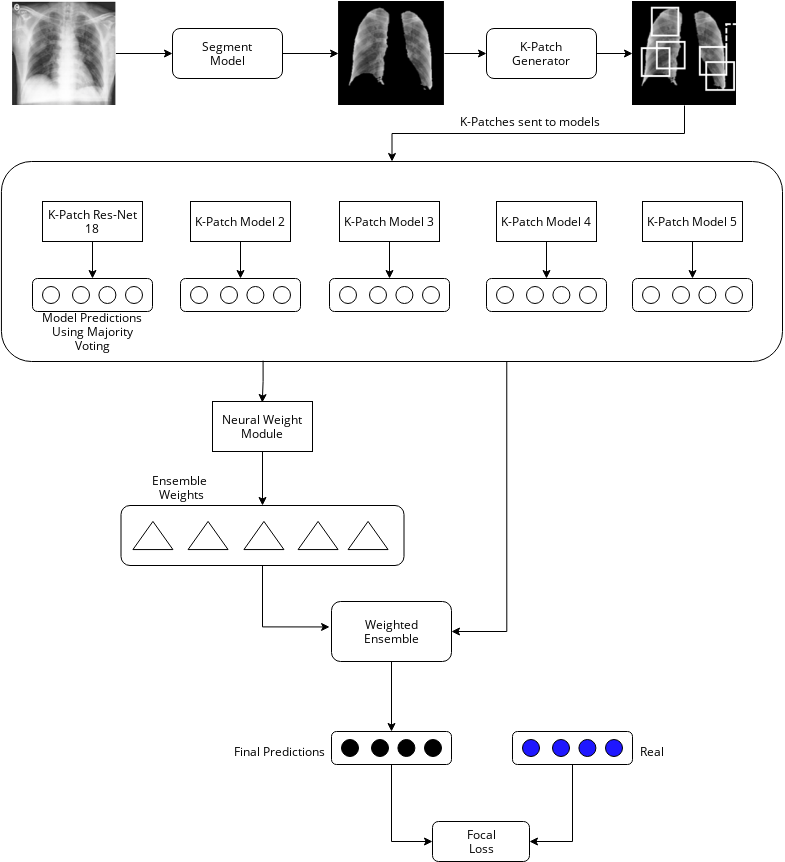
\includegraphics[width=8cm]{../doc/images/FLANNEL-IMPROVED.png}
    \caption{FLANNEL Improvement}
    \label{fig:improve}
\end{figure}

\subsection{Performance Analysis}
We will record the classification accuracy for 4 classes using F1-score. We
compare the F1-score accuracy for COVID-19 vs other classes for five base
learners, FLANNEL with ensemble strategies voting and stacking, FLANNEL with
cross entropy loss, FLANNEL with re-sampling and FLANNEL with k-patch
improvement. We use receiving operating characteristic (ROC) curve and
precision-recall (PR) curve to display classification performance against
threshold. Finally we will provide visual description of FLANNEL and proposed
improvement performance using confusion matrix.

\section{Experimental Setup}
We are planning to use \href{https://github.com/qxiaobu/FLANNEL} {FLANNEL source
    code}  as our baseline and enhance on top of it. Our codebase would be using
    below software/python packages as shown in Table \ref{table:package}
\begin{table}[h]
    \centering
    \caption{Software/Tools used}
    \label{table:package}
    \begin{tabular}{|l|l|} \hline
        Software/Tool & Version \\ \hline
        Python        & 3.8.5   \\ \hline
        numpy         & 1.20.2  \\ \hline
        torch         & 1.8.1   \\ \hline
        torchvision   & 0.9.1   \\ \hline
        matplotlib    & 3.4.0   \\ \hline
        scikit-learn  & 0.24.1  \\ \hline
        pandas        & 1.2.3   \\
        \hline\end{tabular}
\end{table}

As FLANNEL model requires significant compute and GPU resources (3 NVIDIA Tesla
P100 GPUs). We would be utilizing AWS EC2 service with instance type p3.8xlarge
which provides 4 NVIDIA Tesla V100 GPUs along with 32 core CPU and 64GB RAM.

For data analysis and exploration, we are going to use Google Colab.


\begin{figure}[h]
    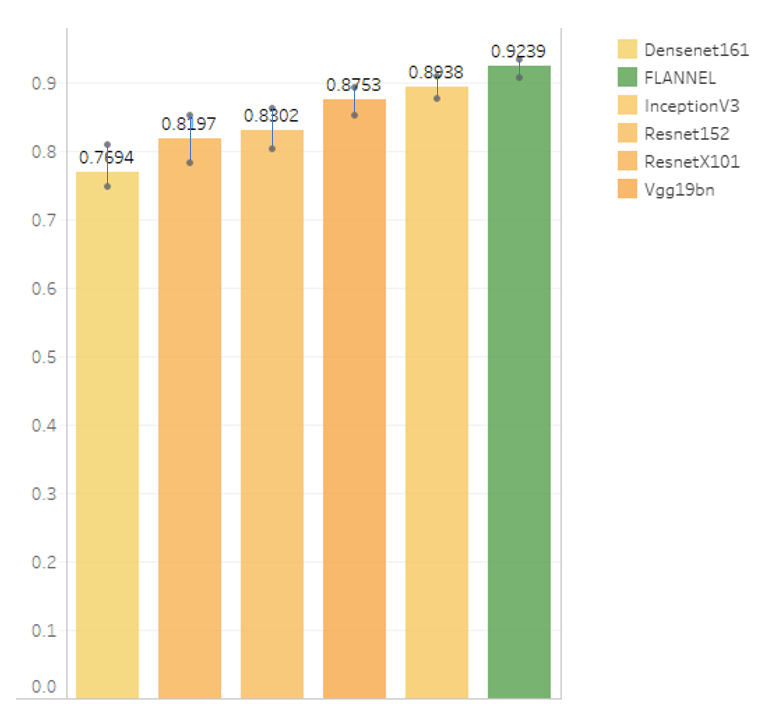
\includegraphics[width=8cm]{../doc/images/F1Score_vs_rest.png}
    \caption{FLANNEL Improvement}
    \label{fig:f1score}
\end{figure}


\begin{figure}[h]
    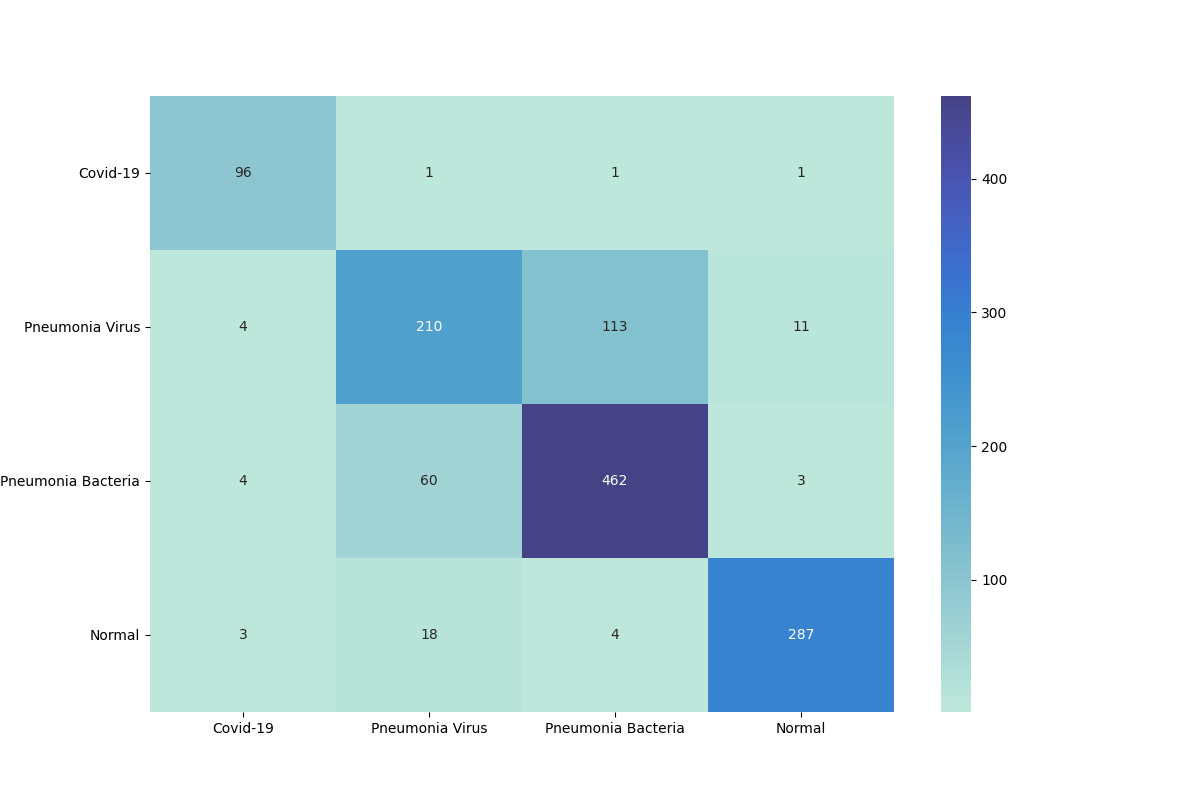
\includegraphics[width=8cm]{../doc/images/confusion_matrix.png}
    \caption{Confusion Matrix}
    \label{fig:cfmatrix}
\end{figure}

\begin{figure}[h]
    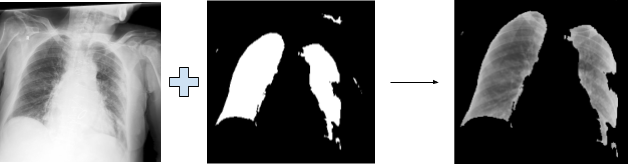
\includegraphics[width=8cm]{../doc/images/segmentation_training.png}
    \caption{Segmentation Training}
    \label{fig:segtrain}
\end{figure}


\newpage
%
% The following two commands are all you need in the initial runs of your .tex
% file to produce the bibliography for the citations in your paper.
\bibliographystyle{abbrv}
\bibliography{covid19}  % sigproc.bib is the name of the Bibliography in this
case

\end{document}
